%% RELATÓRIO DO PROJETO EM JAVA DE LI3

\documentclass[a4paper, 11pt, oneside]{article}

\usepackage[utf8]{inputenc}
\usepackage[T1]{fontenc} 
\usepackage[portuguese]{babel}
\usepackage{graphicx}
\usepackage{hyperref}
\usepackage{xcolor}
\usepackage{multicol}
\usepackage{listingsutf8}


%% DEFINIÇÃO DOS SNIPPETS EM JAVA
\usepackage{listings}
\lstdefinestyle{customc}{
  belowcaptionskip=1\baselineskip,
  breaklines=true,
  language=Java,
  showstringspaces=false,
  basicstyle=\footnotesize\ttfamily,
  keywordstyle=\bfseries\color{green!40!black},
  morekeywords={User, Tag, Post, PostKey},keywordstyle=\bfseries\color{green!40!black},
  commentstyle=\itshape\color{gray},
  stringstyle=\color{orange},
}

\lstset{escapechar=@,style=customc}


%%RELATÓRIO

\begin{document} 

\begin{titlepage}


	\centering 
	
	\scshape
	
	\vspace*{\baselineskip}
	
	
	\rule{\textwidth}{1.6pt}\vspace*{-\baselineskip}\vspace*{2pt}
	\rule{\textwidth}{0.4pt}
	
	\vspace{0.75\baselineskip}
	
	{\LARGE RELATÓRIO DO PROJETO EM JAVA} 
	
	\vspace{0.75\baselineskip} 
	
	\rule{\textwidth}{0.4pt}\vspace*{-\baselineskip}\vspace{3.2pt}
	\rule{\textwidth}{1.6pt}
	
	\vspace{2\baselineskip}
	
	Laboratórios de Informática III
	
	\vspace*{3\baselineskip}
	
	Grupo 24:
	
	\vspace{0.5\baselineskip}
	
	{\scshape\Large Henrique Pereira (a80261) \\ Pedro Moreira (a82364) \\ Pedro Ferreira (a81135) \\}
	
	\vspace{0.5\baselineskip}
	
	\textit{Universidade do Minho \\ Mestrado Integrado em Engenharia Informática}
	
	\vfill

	
\includegraphics[width=40mm]{logoUM.jpg}

	\vspace{0.3\baselineskip}
	
	2018

\end{titlepage}

%% ÌNDICE

\tableofcontents

\newpage

%% INTRODUÇÃO %%%%%%%%%%%%%%%%%%%%%%%%%%%%%%%%%%%%%%%%%%%%%%%%%%%%%%%%%%%%%%%%%%%%%%%%%%%%

\section{Introdução}

No âmbito da unidade curricular \underline{Laboratórios de Informática III}, do 2º ano do Mestrado Integrado em Engenharia Informática, foi-nos proposta a realização de
um projeto que consiste no desenvolvimento de um sistema capaz de processar ficheiros XML, armazenando as várias informações utilizadas pelo Stack Overflow (uma das 
comunidades de perguntas e respostas mais utilizadas atualmente por programadores em todo o mundo). Além disso, após o tratamento da informação, o sistema teria de ser capaz 
de responder eficientemente a um conjunto de interrogações (explicitado na secção \ref{queries}). Esta aplicação teria que ser obrigatoriamente desenvolvida em \textit{Java}.

As estruturas por nós definidas serão apresentadas e justificadas na secção \ref{structs}.

Um ponto fulcral deste trabalho é conciliar a eficiência com o encapsulamento, sem comprometer nenhum destes.




%% ESTRUTURAS %%%%%%%%%%%%%%%%%%%%%%%%%%%%%%%%%%%%%%%%%%%%%%%%%%%%%%%%%%%%%%%%%%%%%%%%%%%%

\newpage
\section{Estrutura}
\label{structs}

Para a realização da segunda fase do projeto tivemos de definir várias classes de dados em \textit{Java}, de maneira a respeitarmos o enunciado, no que toca aos tipos 
concretos e abstratos de dados.



\begin{lstlisting}
	public class TCD implements li3.TADCommunity {
	    private Map<Long, User> users;
	    private Map<PostKey, Post> posts;
	    private Map<Long,String> postAux;
	    private Map<String, Tag> tags;

	    ...
	}
\end{lstlisting}


A nossa decisão de utilizar HashMap vai de encontro ao propósito de aceder diretamente à informação por nós pretendida, no caso de um utilizador, a partir de um ID, no caso
de uma Tag, a partir do seu nome. Porém, para os Posts, decidimos utilizar uma estrutura diferente, neste caso um TreeMap, pois necessitávamos de uma ordem (neste caso 
cronológica) de recolha da informação dos Posts da estrutura que faz uma associação do tipo chave-valor, sendo a ordem dos elementos estabelecida pela comparação das chaves. 
No entanto, sendo os Posts uma unidade central no enunciado proposto, o grupo deparou-se com a necessidade de obter informação relativa a um certo Post, dado o seu \textit{ID}, 
da forma mais eficiente possível. Claramente, realizar uma travessia (\textit{in-order}) na árvore até encontrar o desejado não seria uma boa solução. De forma a otimizar o 
pretendido, foi adicionada à estrutura \textit{TCD} um HashMap cuja chave corresponde ao ID de um Post e o valor armazenado ao \textit{timestamp} do mesmo, considerado até ao 
milissegundo. Deste modo, por comparação de chaves da árvore seria possível efetuar uma procura binária. Contudo verificou-se a exitência de diferentes posts cujos \textit{
timestamps} eram iguais, e a estrutura usada para os armazenar não contempla chaves repetidas. Assim, foi criada a estrutura \textit{postKey}, também esta tornada opaca e 
devidamente encapsulada, apenas contendo a data e o ID de um Post, que passou a ser usada como chave de inserção na árvore. Desta forma garantiu-se não só a ordenação pretendida 
como a unicidade de cada uma das chaves. No caso de dois Posts terem o mesmo \textit{timestamp}, considerou-se como sendo maior o Post com menor ID. Para efeitos de procura de 
um Post, foi criada a função \textit{getPost}, cuja execução se divide nas duas tarefas descritas anteriormente: dado o ID de um Post, criar uma variável do tipo 
\textit{postKey}, com o ID e o \textit{timestamp} presente na tabela de Hash \textit{postAux} e, de seguida, proceder a uma procura binária na árvore dos Posts.


\begin{lstlisting}
	public class User {	
	    private long id;
	    private String display_name;
	    private int n_posts;
	    private int reputacao;
	    private String short_bio;
	    private Set<Post> user_posts;

	    ...
	}
\end{lstlisting}

\begin{lstlisting}
	public class Post {
	    private long id;
	    private String titulo;
	    private long owner_id;
	    private int type_id;
	    private long parent_id;
	    private LocalDateTime data;
	    private List<Tag> tags;
	    private int score;
	    private int n_comments;
	    private int n_answers;

	    ...
	}
\end{lstlisting}

\begin{lstlisting}
	public class PostKey implements Comparable<PostKey>{
	    private LocalDateTime data;
	    private long id;

	    ...
	}
\end{lstlisting}

\begin{lstlisting}
	public class Tag {
	    private String nome;
	    private long id;

	    ...
	}
\end{lstlisting}



%% QUERIES

%% Interrogações e Abordagem %%%%%%%%%%%%%%%%%%%%%%%%%%%%%%%%%%%%%%%%%%%%%%%%%%%%%%%%%%%%%%%%%%%%%%%%%%%%

\section{Interrogações e Abordagem}

\label{queries}
Nesta secção, iremos explicitar a nossa abordagem às interrogações descritas no enunciado,
desta vez na linguagem \textit{Java}.


A primeira funcionalidade da aplicação que tivemos que implementar foi o carregamento dos dados a partir dos ficheiros XML. Para tal, assumimos uma abordagem diferente daquela que apresentamos aquando da primeira fase do Projeto em \textit{C}. Isto porque, em vez de carregarmos os documentos todos para a memória, o que seria uma má implementação para ficheiros de grande tamanho, decidimos utilizar a API do Java que permite este carregamento, mas de uma maneira faseada, ou seja, por blocos. A API utilizada foi, portanto, o \texttt{StAX} (\textit{Streaming API for XML}), que permite parsing de ficheiros XML através de \textit{streaming}. Preferimos o \texttt{StAX} face ao \texttt{SAX} pela facilidade de utilização do primeiro.

Assim sendo, utilizando esta API, fizemos o carregamento dos dados presentes no ficheiros XML para as nossas estruturas, de forma a podermos responder às várias \textit{queries} apresentadas.


%% QUERY 1
\subsection{Info From Post}

A resolução da primeira \textit{query} foi semelhante à estratégia adotada no projeto anterior. Através do método \textit{getPost}, presente na classe \textit{TCD}, tentamos aceder à informação relativa ao \textit{ID} passado como paramêtro. Caso o \textit{post} não exista, é lançada uma exceção que alertará o utilizador para a situação (\textit{PostNotFoundException}). Caso contrário é efetuada uma tentativa de aceder às informações do criador do \textit{post}, através do método \textit{getUser}, ou é repetido o processo caso o \textit{post} seja uma resposta, desta vez, procurando dados sobre a respetiva pergunta. 


%% QUERY 2
\subsection{Top Most Active}

Para obter a resposta desejada utilizamos como estrutura intermédia um \textit{TreeSet} criado através do seu construtor que permite que lhe seja passado um critério de ordenação como paramêtro. Para tal efeito, recorremos a uma \textit{lambda expression} de forma a suprimir a necessidade de criar uma classe especificamente para se declarar um novo comparador ou usar uma classe interna anónima, cuja leitura é complicada. De seguida inserimos todos os utilizadores nesta árvore através do método \textit{addAll}, e procedemos ao tratemento dos dados sobre a forma de \textit{stream}. Limitamos os elementos da mesma ao número de utilizadores que pretendemos obter e, de seguida, alteramos o tipo dos dados a circular na \textit{stream} para os seus \textit{ID's}, inserindo-os numa lista de imediato.



%% QUERY 3
\subsection{Total Posts}



%% Comparação das duas versões


%% QUERY 4
\subsection{Questions with Tag}

Mais uma vez, a estratégia usada guia-se pelas construções funcionais disponibilizados no \textit{Java 8}. A resolução passa por fazer \textit{stream} dos \textit{post's}, reter apenas aqueles que ocorreram no intervalo de datas passado como parâmetro e que contenham a tag dada. De seguida, finalizamos colecionando os \textit{ID's} dos mesmo para uma lista.


%% QUERY 5
\subsection{Get User Info}

Esta \textit{query} tem resolução quase imediata. Simplesmente acedemos à informação respetiva ao utilizador cujo \textit{ID} foi passado como argumento, sendo lançada a respetiva exceção caso este nao exista. Obtemos os seus últimos dez \textit{post's} recorrendo ao mecanismo funcional e por fim montamos o resultado.

%% QUERY 6
\subsection{Most Voted Answers}

Para solucionar esta \textit{query} criamos um \textit{TreeSet} cujo critério de ordenação tem por base o \textit{Score} dos \textit{post's} que lá vão ser inseridos. Como critério de desempate, utilizamos a ordem crescente dos \textit{ID's}. Posteriormente, todas as respostas ocorridas entre as datas passadas como argumento são inseridas no mesmo. Para finalizar, retiramos os N primeiros elementos do \textit{TreeSet} e construimos uma lista com os seus \textit{ID's}.


%% QUERY 7

A resolução desta \textit{query} é em tudo identicâ à da \textit{query} anterior, à excepção do critério de ordenação usado no \textit{TreeSet}. Neste caso, o \textit{TreeSet} é populado apenas com perguntas, cuja ordem é estabelecida pelo número de respostas que estas obtiveram.

\begin{lstlisting}
	public List<Long> mostAnsweredQuestions(int N, LocalDate begin, LocalDate end);
\end{lstlisting}



%% QUERY 8
\subsection{Contains Word}

Através das construções funcionais a resolução desta \textit{query} tornou-se bastante simples, e a sua leitura altamente simplificada em relação à implementação realizada em \textit{C}. Apenas foi preciso fazer \textit{stream} dos \textit{posts} e filtrar as perguntas cujo título continha a palavra passada como argumento. Para tal, usamos o método \textit{contains} presente em \textit{java.lang.String}. Novamente, limitamos o número de elementos na \textit{stream} ao tamanho que foi passado como argumento e colecionamos o resultado.



%% QUERY 9
\subsection{Both Participated}

De forma a chegar ao resultado correto, procedemos, tal como no projeto anterior, à evocação de um método auxiliar sobre a coleção de \textit{posts} de ambos os utilizadores passados como argumento. Esse método troca todas as ocorrências de respostas pelas respetivas perguntas. Deste modo, é nos possivel intercetar os \textit{posts} em que ambos particaparam recorrendo simplesmente ao método \textit{retainAll}. Para finalizar, colecionamos, no máximo, os N \textit{ID's} de \textit{posts} que estes tenham em comum.

%% QUERY 10
\subsection{Better Answer}

Nesta \textit{query} recorremos novamente à utilização de um \textit{TreeSet} como estrutura de ordenação, inserido os candidatos a resposta aquando do fecho de uma \textit{stream} de todos os \textit{posts}, filtrada para conter apenas as respostas à pergunta cujo \textit{ID} foi passado como argumento. No caso de essa pergunta não existir ou não ter resposta são lançadas as devidas exceções. Caso contrário é retornado o \textit{ID} do primeiro elemento da árvore.



%% QUERY 11
\subsection{Most Used Best Rep}

A abordagem à décima primeira (e última) \textit{query} pode-se dividir em três fases. Numa primeira fase, é montada uma lista com todas as \textit{tags} usadas no intervalo de tempo em causa (incluindo repetições, dado que é fundamental para o próximo passo). De seguida é criado um \textit{Map} cujas chaves correspondem ao \textit{ID} de uma \textit{tag} e o valor ao número de ocorrências da mesma. Esta tarefa foi bastante simplicada fazendo uso dos métodos \textit{groupingBy} e \textit{couting} presentes em  \textit{java.util.stream.Collectors}. 






%% RESULTADOS %%%%%%%%%%%%%%%%%%%%%%%%%%%%%%%%%%%%%%%%%%%%%%%%%%%%%%%%%%%%%%%%%%%%%%%%%%%%%%%
\section{Resultados}

\subsection{Análise dos resultados}

\begin{table}[h] 
	\centering
	\caption{Tempo (ms) - Ubuntu}	
	\begin{tabular}{c|c|c}
	Interrogação: & Input nº1:      & Input nº2:      \\
	1             & 0.01            & 0.01            \\
	2             & 198.0           & 197.0           \\
	3             & 50.0            & 54.0            \\
	4             & 47.0            & 47.0            \\
	5             & 1.0             & 1.0             \\
	6             & 39.0            & 42.0            \\
	7             & 43.0            & 48.0            \\
	8             & 7.0             & 11.0            \\
	9             & 2.0             & 0.0             \\
	10            & 28.0            & 28.0            \\
	11            & 182.0           & 198.0  
	\end{tabular}
\end{table}



\subsection{Comparação dos Resultados}

De forma a ser mais fácil comparar os resultados obtidos com as nossas abordagens em \textit{C} e \textit{Java},
desenvolvemos os gráficos \ref{graphLoad}, \ref{graphQs1} e \ref{graphQs2}, que representam os tempos de execução do carregamento dos dados (\texttt{load}) e das \textit{queries} (um gráfico para cada \textit{input}, respetivamente.


Como podemos ver pelo gráfico \ref{graphLoad}, os tempos de execução do \texttt{load} do \textit{Java} são inferiores aos do \textit{C}, sendo que esta diferença é mais díspar quando executamos o carregamento do \textit{dump} do Ubuntu. Podemos observar que os tempos do Java para o Android e Ubuntu são de 2 segundos e 12 segundos, respetivamente, enquanto que os do C são, para os mesmos \textit{dumps}, de 3 e 19 segundos.

Os gráficos \ref{graphQs1} e \ref{graphQs2} mostram-nos o seguinte:
\begin{itemize}
\item Na \textit{Query} 1, na \textit{Query} 5 e na \textit{Query} 9, ambos os tempos de execução da aplicação em C e Java são muito reduzidos, quando comparados com os resultados das outras interrogações.
\item As \textit{Queries} 2 e 11, são as únicas interrogações onde o tempo de execução em Java é superior ao tempo de execução em C em cerca de 50 milissegundos. No input 1, podemos verificar também um ligeiro aumento do tempo da aplicação em Java perante o tempo daquela em C.
\item Os tempos de execução das restantes \textit{Queries} mostram que o desempenho da aplicação em Java é bastante superior à em C, diferença esta mais denotada nas interrogações 4, 8 e 10. Os resultados dos dois inputs divergem, sendo que os tempos em C são imensamente maiores no segundo input, enquanto que os tempos em Java se mantêm.
\end{itemize}

\begin{figure}[h]
\centering
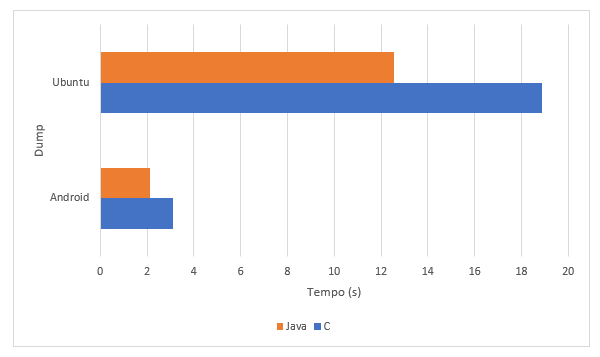
\includegraphics[scale=.5]{loads.png}
\caption{Tempos de Execução - Load \label{graphLoad}}
\end{figure}

\begin{figure}[h] 
\centering
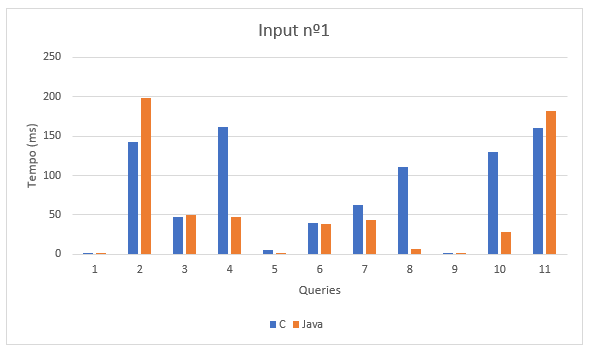
\includegraphics[scale=.5]{input_1.png}
\caption{Tempos de Execução - Queries (Input 1) \label{graphQs1}}
\end{figure}

\begin{figure}[h] 
\centering
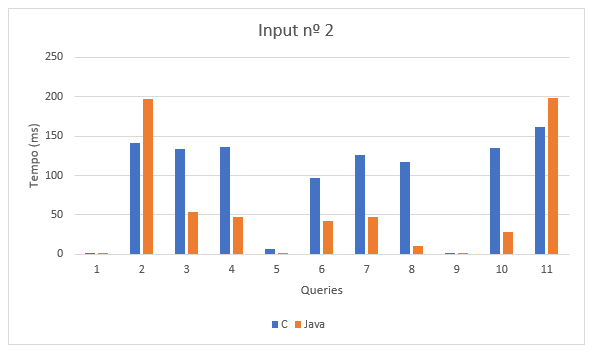
\includegraphics[scale=.5]{input_2.png}
\caption{Tempos de Execução - Queries (Input 2) \label{graphQs2}}
\end{figure}

\newpage
%% CONCLUSÃO %%%%%%%%%%%%%%%%%%%%%%%%%%%%%%%%%%%%%%%%%%%%%%%%%%%%%%%%%%%%%%%%%%%%%%%%%%%%%%%%
\section{Conclusão}


%%  DIZER QUAL O MELHOR !-!-!-!-!-!-!-!-!-!-!-!-!-!-!-!-!-!-!-!-!-!-!-!-!-!-!-!-!-!-!-!-!-!-!-!-!-!-!-!-!-!-!-!-!-!


Este projeto foi extremamente enriquecedor para o grupo, uma vez que nos permitiu trabalhar com um tipo diferente de dados, o XML, e nos ensinou a trabalhar com ele. 
Tivemos que nos esforçar bastante para conseguirmos atingir os objetivos estabelecidos, tendo sempre em atenção o encapsulamento do código e a sua eficiência. O trabalho 
permitiu-nos também aprender a desenvolver as estruturas de que precisamos, consoante as dificuldades, exigências e necessidades que nos foram sendo impostas com o 
desenrolar do projeto.

Os resultados que obtivemos, ao correr o programa, foram iguais aos dos testes fornecidos pelos docentes,
pelo que podemos concluir que a nossa implementação está correta.
Além disso, achamos que cumprimos o objetivo de criar um programa eficiente,
visto que os tempos que obtivemos para cada interrogação, utilizando os \textit{dumps} do
Ubuntu e os mesmos parâmetros utilizados pelos professores nos testes, foram os seguintes (aproximadamente):


Em suma, tendo em conta a eficiência e os resultados que obtivemos, podemos concluir
que conseguimos atingir as metas propostas com este projeto, dado que os tempos de
execução, tanto do \textit{load} como das interrogações, foram bastante positivos.
Com os \textit{getters} e \textit{setters} por nós definidos para as nossas estruturas,
conseguimos sempre, com a modulação e separação dos ficheiros que fizemos, respeitar o encapsulamento da informação.
\end{document}
